% NTG_Picture22a
% Nathan Gray

\documentclass[10pt]{standalone}
\usepackage{amsmath}
\usepackage{tikz}
\usetikzlibrary{hobby}
\usepackage{tkz-euclide}


\begin{document}
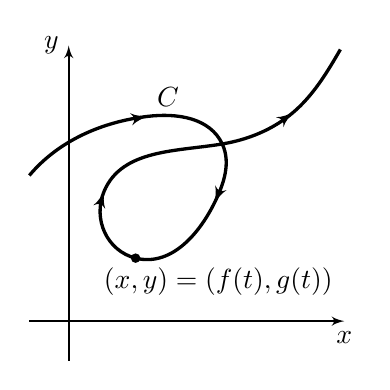
\begin{tikzpicture}[>=latex']
% x-axis
\draw[semithick, ->] (-0.5, 0) -- (3.5, 0) node[below] {$x$};
% y-axis
\draw[semithick, ->] (0, -0.5) -- (0, 3.5) node[left] {$y$};	
% Coordinates of points on curve
\coordinate (a1) at (-0.5,1.85);
\coordinate (a2) at (1,2.6);
\coordinate (a3) at (1.95,2.25);
\coordinate (a3b) at (1.85,1.5);
\coordinate (a4) at (0.85,0.8);
\coordinate (a5) at (0.45,1.65);
\coordinate (a6) at (2.85,2.65);
\coordinate (a7) at (3.45,3.45);
% Plot point
\filldraw[black] (a4) circle(1.5pt);
\node[below] at (1.9,0.8) {$(x,y) = (f(t),g(t))$};
% Plot curve C
\draw[black, very thick, use Hobby shortcut] ([out angle=50]a1) .. (a2) .. (a3) .. (a3b) .. (a4) .. (a5) .. (a3) .. (a6) .. ([in angle=240]a7);
\node[above right] at (a2) {$C$};
% Arrows
%
% (There is likely an easier way to draw the curve C that will include the arrows, i.e., a way that uses the Hobby library and puts the arrows at some of the specific points on C.)
\node[rotate=-80, scale=1.5] at (a2) {\tikz\draw[-latex', black] (a2);}; 
\node[rotate=157, scale=1.5] at (a3b) {\tikz\draw[-latex', black] (a3b);}; 
\node[rotate=-17, scale=1.5] at (a5) {\tikz\draw[-latex', black] (a5);}; 
\node[rotate=-54, scale=1.5] at (a6) {\tikz\draw[-latex', black] (a6);}; 
\end{tikzpicture}
\end{document}

